\documentclass{ximera}

\title{Kinetiek modelleren met Machine Learning}
\author{Mila Vervoort}
\license{CC: 0}         % replace with an appropriate license, or set it in xmPreamble

\begin{document}
\begin{abstract}
    Een introductie over Machine Learning en Neurale Netwerken voor het toepassen op reactorkunde
\end{abstract}
\maketitle
\label{xim:Machine Learning}

\section*{Waarom Machine Learning?}

In de reactorkunde worden reactoren doorgaans beschreven met wiskundige modellen die gebaseerd zijn op de fysische en chemische processen die in het systeem plaatsvinden. Wanneer de onderliggende processen goed gekend zijn, kunnen bijvoorbeeld massabalansen en reactiesnelheidsvergelijkingen worden opgesteld om het gedrag van de reactor te beschrijven.

Deze aanpak is bijzonder krachtig wanneer de fysische en chemische processen voldoende gekend zijn. Zo kunnen we op basis van een gekend reactiemechanisme een geschikte reactiesnelheidsvergelijking opstellen en vervolgens de bijbehorende kinetische parameters bepalen uit experimentele gegevens.

In de praktijk is onze kennis van een reactiesysteem echter niet altijd volledig. Een systeem kan bijvoorbeeld meerdere gelijktijdige reacties, tussenproducten en nevenreacties bevatten. Ook kunnen bepaalde reactiemechanismen onvoldoende gekend zijn of kunnen niet alle relevante variabelen experimenteel worden gemeten. Het kan dan moeilijk zijn om vooraf een wiskundig model op te stellen dat het volledige gedrag van het systeem correct beschrijft.

We beschikken in dergelijke situaties vaak wel over experimentele gegevens. Deze gegevens bevatten informatie over hoe het systeem zich gedraagt, ook wanneer de onderliggende mechanismen niet volledig gekend zijn. Dit maakt het interessant om niet alleen vanuit onze fysische kennis te vertrekken, maar ook gebruik te maken van de informatie die in de gegevens aanwezig is. Dit vormt het uitgangspunt van \textbf{Machine Learning}. 

\begin{conclusion} \text{ }

Bij Machine Learning wordt een model gebruikt waarvan de parameters worden geleerd uit beschikbare gegevens. Het model probeert hierbij verbanden en patronen in de gegevens te leren, zodat het vervolgens voorspellingen kan maken voor nieuwe situaties. 

\begin{center}
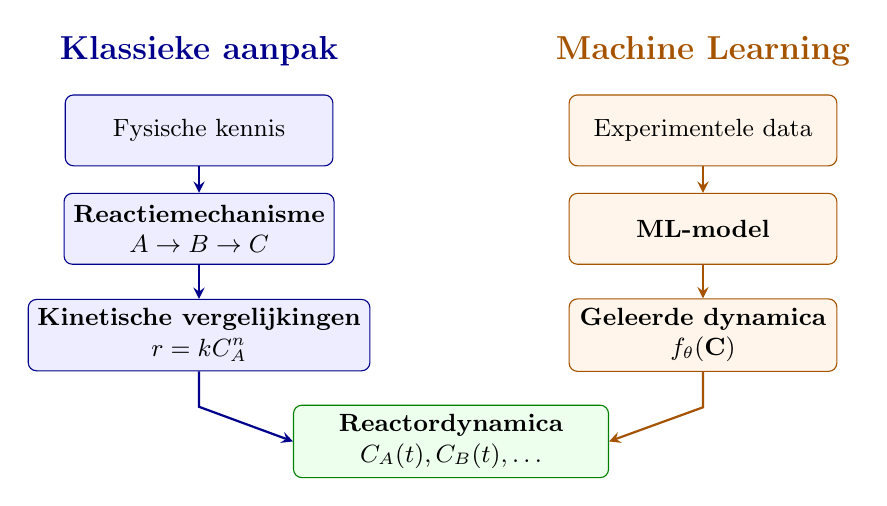
\begin{tikzpicture}[
    >=stealth,
    font=\small,
    box/.style={
        draw,
        rounded corners=3pt,
        minimum width=3.4cm,
        minimum height=0.9cm,
        align=center
    },
    classic/.style={
        box,
        fill=blue!7,
        draw=blue!55!black
    },
    machine/.style={
        box,
        fill=orange!8,
        draw=orange!65!black
    },
    arrow/.style={
        ->,
        thick
    }]

% Titels
\node[
    font=\bfseries\large,
    text=blue!55!black
] at (-3.2,4.6)
{Klassieke aanpak};

\node[
    font=\bfseries\large,
    text=orange!65!black
] at (3.2,4.6)
{Machine Learning};


% Input
\node[classic] (physics) at (-3.2,3.6)
{Fysische kennis};

\node[machine] (data) at (3.2,3.6)
{Experimentele data};


% Tweede blok
\node[classic] (mechanism) at (-3.2,2.35)
{\textbf{Reactiemechanisme}\\
$A\rightarrow B\rightarrow C$};

\node[machine] (ml) at (3.2,2.35)
{\textbf{ML-model}};


% Derde blok
\node[classic] (kinetics) at (-3.2,1.0)
{\textbf{Kinetische vergelijkingen}\\
$r=kC_A^n$};

\node[machine] (dynamics) at (3.2,1.0)
{\textbf{Geleerde dynamica}\\
$f_\theta(\mathbf C)$};


% Pijlen
\draw[arrow, blue!55!black]
(physics) -- (mechanism);

\draw[arrow, blue!55!black]
(mechanism) -- (kinetics);

\draw[arrow, orange!65!black]
(data) -- (ml);

\draw[arrow, orange!65!black]
(ml) -- (dynamics);


% Output
\node[
    draw=green!50!black,
    fill=green!7,
    rounded corners=3pt,
    minimum width=4.0cm,
    minimum height=0.75cm,
    align=center,
    font=\small
] (output) at (0,-0.35)
{\textbf{Reactordynamica}\\
$C_A(t),C_B(t),\ldots$};


% Pijlen naar gezamenlijke output
\draw[arrow, blue!55!black]
(kinetics.south)
-- ++(0,-0.45)
-- (output.west);

\draw[arrow, orange!65!black]
(dynamics.south)
-- ++(0,-0.45)
-- (output.east);

\end{tikzpicture}
\end{center}
\end{conclusion}

\begin{remark} \text{ }

    Machine Learning hoeft hierbij geen vervanging te zijn voor de klassieke fysische modellen. In veel toepassingen kunnen fysische kennis en Machine Learning juist worden gecombineerd. Zo kan de fysische structuur van een probleem vooraf worden vastgelegd, terwijl een Machine Learning-model wordt gebruikt om een onbekend of moeilijk te beschrijven onderdeel uit de experimentele gegevens te leren.
\end{remark} \text{ }

\section*{Wat is Machine Learning?}

Machine Learning is een verzameling technieken waarmee een model uit
gegevens kan worden geleerd. In plaats van een model volledig vooraf vast te leggen, worden de parameters van het model bepaald op basis van beschikbare gegevens. Het doel is om een model te verkrijgen dat verbanden in de gegevens kan beschrijven en vervolgens voorspellingen kan maken voor nieuwe situaties.

Een eenvoudig Machine Learning-probleem kan schematisch worden voorgesteld
als

\[
x
\quad\longrightarrow\quad
\boxed{f_\theta}
\quad\longrightarrow\quad
\hat{y},
\]

waarbij $x$ de invoer van het model is, $\hat{y}$ de voorspelling van het
model en $f_\theta$ het model zelf voorstelt. De index $\theta$ geeft aan dat
het model afhankelijk is van een verzameling parameters $\theta$.

De voorspelling kan daarom worden geschreven als

\[
\hat{y}=f_\theta(x).
\]

De letter $y$ wordt gebruikt voor de werkelijke of gewenste uitvoer. Het
hoedje in $\hat{y}$ geeft aan dat het om een voorspelling gaat.

\begin{remark} \textbf{Verschillende vormen van Machine Learning}

Machine Learning kan op verschillende manieren worden toegepast, afhankelijk
van de beschikbare gegevens en het doel van het model. Een belangrijk
onderscheid wordt gemaakt tussen supervised learning,
unsupervised learning en reinforcement learning.

\begin{itemize}
    \item Bij \textbf{supervised learning} beschikt men over voorbeelden waarbij zowel de invoer $x$ als de bijbehorende gewenste uitvoer $y$ gekend zijn. Het model leert op basis van deze voorbeelden een verband tussen de invoer en de uitvoer.
    Binnen supervised learning wordt een onderscheid gemaakt tussen regressie en classificatie. \\
    Bij \textbf{regressie} probeert het model een continue grootheid te
    voorspellen. De uitvoer kan bijvoorbeeld een temperatuur, concentratie of reactiesnelheid zijn. Het model leert dan bijvoorbeeld een verband van de vorm $\hat{y}=f_\theta(x).$ \\
    Bij \textbf{classificatie} probeert het model een observatie toe te wijzen aan één van een aantal categorieën of klassen. De uitvoer is dan geen continue grootheid, maar bijvoorbeeld "A", "B" of "C", of een binaire klasse zoals "ja" of "nee".

    \item Bij \textbf{unsupervised learning} zijn er geen vooraf gegeven doelwaarden $y$. Het model krijgt enkel de beschikbare gegevens en probeert hierin zelf structuren of patronen te vinden. Een voorbeeld hiervan is clustering, waarbij gelijkaardige gegevenspunten automatisch in groepen worden verdeeld.

    \item Bij \textbf{reinforcement learning} leert een model door interactie met een omgeving. Het model voert acties uit en ontvangt hiervoor een beloning of straf. Op basis van deze ervaringen leert het model welke acties tot een gewenst resultaat leiden.
\end{itemize}

In deze cursus richten we ons voornamelijk op supervised learning, en meer specifiek op regressie. We beschikken immers over experimentele gegevens en willen daaruit continue grootheden, zoals reactiesnelheden en
concentraties, leren voorspellen.
\end{remark}

\section*{Trainen van een model via Supervised Learning}

Bij supervised learning leert het model uit voorbeelden waarvoor zowel de invoer als de gewenste uitvoer gekend zijn. Eén voorbeeld bestaat uit een invoer $x$ en de bijbehorende gewenste uitvoer $y$:

\[
(x,y).
\]

Dit wordt een trainingsvoorbeeld genoemd.

Wanneer meerdere trainingsvoorbeelden beschikbaar zijn, vormen deze samen de trainingsset. 

\begin{definition} \textbf{Trainingsset}
    
Een trainingsset met $m$ voorbeelden kan worden
geschreven als

\[
\mathcal{D}
=
\left\{
(x^{(1)},y^{(1)}),
(x^{(2)},y^{(2)}),
\ldots,
(x^{(m)},y^{(m)})
\right\}.
\]

Hierbij stelt $i$ het nummer van een trainingsvoorbeeld voor en is $m$ het
totale aantal voorbeelden in de trainingsset.

De grootheden in $x$ worden de \textbf{features} of
\textbf{inputvariabelen} genoemd. De bijbehorende waarde $y$ wordt de
\textbf{target} of \textbf{doelwaarde} genoemd.
\end{definition}

\begin{example} \textbf{Reactiesnelheid voorspellen}

Een eenvoudig voorbeeld uit de reactorkunde is het voorspellen van een
reactiesnelheid op basis van concentraties. Stel dat voor verschillende
toestanden van een reactiesysteem de concentraties $C_A$, $C_B$ en $C_C$ en de
bijbehorende reactiesnelheid $r$ gekend zijn. Eén trainingsvoorbeeld kan dan
worden geschreven als

\[
x=
\begin{bmatrix}
C_A\\
C_B\\
C_C
\end{bmatrix},
\qquad
y=r.
\]

De concentraties zijn hierbij de features van het voorbeeld en de
reactiesnelheid is de target. Voor meerdere experimentele
toestanden ontstaat een trainingsset met verschillende combinaties van
concentraties en bijbehorende reactiesnelheden.

Het Machine Learning-model probeert op basis van deze voorbeelden een functie
te leren van de vorm

\[
\hat{r}=f_\theta(C_A,C_B,C_C).
\]

Wanneer het model vervolgens een nieuwe combinatie van concentraties krijgt,
kan het met behulp van deze geleerde relatie een reactiesnelheid voorspellen.

\end{example} \text{ }

\subsection{Het trainingsproces}

Het doel van het trainen van een supervised-learningmodel is om de parameters $\theta$ zo te bepalen dat het model goede voorspellingen maakt voor de beschikbare trainingsgegevens. Dit gebeurt door de voorspellingen van het
model systematisch te vergelijken met de bekende targetwaarden.

Het trainingsproces kan schematisch worden weergegeven als
\[
\boxed{
\text{invoer}
\rightarrow
\text{voorspelling}
\rightarrow
\text{loss}
\rightarrow
\text{kostfunctie}
\rightarrow
\text{gradiënt}
\rightarrow
\text{parameterupdate}
}
\]

Deze stappen worden herhaald totdat de optimalisatie een geschikt resultaat oplevert.

Tijdens het trainen beschikt het model dus over trainingsvoorbeelden
$(x^{(i)},y^{(i)})$. Voor ieder voorbeeld maakt het model op basis van zijn
huidige parameters een voorspelling:

\[
\hat{y}^{(i)}
=
f_\theta(x^{(i)}).
\]

Deze voorspelling wordt vergeleken met de bijbehorende target $y^{(i)}$. \\
Het verschil tussen de voorspellingen en de targetwaarden wordt beschreven
met een lossfunctie en kostfunctie.

\begin{definition} \textbf{Lossfunctie en Kostfunctie}

\textbf{De lossfunctie} geeft aan hoe goed het model
de beschikbare gegevens beschrijft.

Een veelgebruikte lossfunctie voor regressie is de Mean Squared Error (MSE).
Voor één trainingsvoorbeeld wordt de fout gegeven door

\[
L^{(i)}
=
\left(
y^{(i)}-\hat{y}^{(i)}
\right)^2.
\]

Om de prestaties van het model over de volledige trainingsset van $m$ voorbeelden te beoordelen, nemen we het gemiddelde van deze fouten. Dit resulteert in de \textbf{kostfunctie}

\[
J(\theta)
=
\frac{1}{m}
\sum_{i=1}^{m}
\left(
y^{(i)}-\hat{y}^{(i)}
\right)^2.
\]

De kostfunctie geeft dus de gemiddelde fout van het model over alle trainingsvoorbeelden weer.
\end{definition}

Het doel van de training is om de parameters $\theta$ zo te kiezen dat de
kostfunctie zo klein mogelijk wordt:

\[
\boxed{
\theta^*
=
\underset{\theta}{\operatorname{arg\,min}}\;J(\theta)
}
\]

Dit is vergelijkbaar met het principe van de kleinste-kwadratenmethode, waarbij parameters worden gekozen om
gekwadrateerde afwijkingen tussen voorspellingen en metingen te
minimaliseren.

Bij Machine Learning kan het aantal parameters echter groot zijn. Daarom worden de parameters meestal iteratief aangepast met behulp van een optimalisatiemethode. Een veelgebruikte methode is
\textbf{gradient descent}. Hierbij wordt de gradiënt van de kostfunctie
gebruikt om de parameters aan te passen:

\[
\theta_{k+1}
=
\theta_k
-
\eta
\nabla_\theta J(\theta_k)
\]

Hierbij is $\eta$ de \textbf{learning rate}, die bepaalt hoe groot de
parameterstap is. De parameters worden dus steeds aangepast in de richting
waarin de kostfunctie afneemt.

In de praktijk wordt vaak een variant van gradient descent gebruikt, zoals
\textbf{Adam}. Adam houdt naast de huidige gradiënt ook informatie bij over
eerdere gradiënten, waardoor de grootte van de parameterupdates automatisch
kan worden aangepast. Hierdoor kan de optimalisatie efficiënter verlopen.

\begin{conclusion} \text{ }

Het leerproces kan schematisch worden samengevat als

\[
\boxed{
\text{voorspelling}
\rightarrow
\text{loss berekenen}
\rightarrow
\text{gradiënt bepalen}
\rightarrow
\text{parameters aanpassen}
}
\]

Dit proces wordt herhaald totdat de kostfunctie voldoende klein is.

\end{conclusion}

\section*{Wat is Machine Learning?}

Machine Learning is een verzameling technieken waarmee een model uit gegevens
kan worden geleerd. In plaats van een model volledig vooraf vast te leggen,
worden de parameters van het model bepaald op basis van beschikbare gegevens.
Het doel is om een model te verkrijgen dat verbanden in de gegevens kan
beschrijven en vervolgens voorspellingen kan maken voor nieuwe situaties.

Een eenvoudig Machine Learning-probleem kan schematisch worden voorgesteld
als

\[
x
\quad\longrightarrow\quad
\boxed{f_\theta}
\quad\longrightarrow\quad
\hat{y},
\]

waarbij $x$ de invoer van het model is, $\hat{y}$ de voorspelling van het
model en $f_\theta$ het model voorstelt. De index $\theta$ geeft aan dat het
model afhankelijk is van een verzameling parameters $\theta$.

De voorspelling kan daarom worden geschreven als

\[
\hat{y}=f_\theta(x).
\]

De letter $y$ wordt gebruikt voor de werkelijke of gewenste uitvoer. Het
hoedje in $\hat{y}$ geeft aan dat het om een voorspelling gaat.

\begin{remark} \textbf{Verschillende vormen van Machine Learning}

Machine Learning kan op verschillende manieren worden toegepast, afhankelijk
van de beschikbare gegevens en het doel van het model.

Bij \textbf{supervised learning} beschikt men over voorbeelden waarbij zowel
de invoer $x$ als de bijbehorende gewenste uitvoer $y$ gekend zijn. Het model
leert op basis van deze voorbeelden een verband tussen de invoer en de
uitvoer. Bij \textbf{regressie} is de gewenste uitvoer een continue
grootheid, terwijl bij \textbf{classificatie} de uitvoer bestaat uit één van
een aantal categorieën.

Bij \textbf{unsupervised learning} zijn er geen vooraf gegeven doelwaarden
$y$. Het model probeert zelf structuren of patronen in de gegevens te vinden.
Een voorbeeld hiervan is clustering, waarbij gelijkaardige gegevenspunten in
groepen worden verdeeld.

Bij \textbf{reinforcement learning} leert een model door interactie met een
omgeving. Het model voert acties uit en ontvangt hiervoor een beloning of
straf. Op basis hiervan leert het model welke acties tot een gewenst resultaat
leiden.

In deze cursus richten we ons voornamelijk op problemen waarbij we uit
experimentele gegevens continue grootheden willen voorspellen. We behandelen
daarmee voornamelijk regressieproblemen.
\end{remark}

\begin{example} \textbf{Reactiesnelheid voorspellen}

Een voorbeeld uit de reactorkunde is het voorspellen van een reactiesnelheid
op basis van concentraties. Stel dat voor verschillende toestanden van een
reactiesysteem de concentraties $C_A$, $C_B$ en $C_C$ en de bijbehorende
reactiesnelheid $r$ gekend zijn.

Eén voorbeeld kan dan worden voorgesteld als

\[
x=
\begin{bmatrix}
C_A\
C_B\
C_C
\end{bmatrix},
\qquad
y=r.
\]

De concentraties zijn hierbij de \textbf{features} of inputvariabelen en de
reactiesnelheid is de \textbf{target} of doelwaarde.

Voor meerdere experimentele toestanden ontstaat een verzameling van dergelijke
voorbeelden. Het model probeert op basis hiervan een verband te leren van de
vorm

\[
\hat{r} = f_\theta(C_A,C_B,C_C).
\]

Wanneer het model vervolgens een nieuwe combinatie van concentraties krijgt,
kan het met behulp van deze geleerde relatie een reactiesnelheid voorspellen.
\end{example}

\section*{Het Machine Learning-proces}

Om van beschikbare gegevens tot een bruikbaar model te komen, worden
verschillende stappen doorlopen:

\[
\boxed{
\begin{array}{c}
\text{Gegevens verzamelen}\\
\downarrow \\
\text{Gegevens voorbereiden en opsplitsen}\\
\downarrow \\
\text{Model kiezen}\\
\downarrow \\
\text{Model trainen}\\
\downarrow\\
\text{Model evalueren}\\
\end{array}
}
\]

Deze stappen worden hieronder verder toegelicht.

\begin{itemize}
\item \textbf{Gegevens verzamelen en voorbereiden}

Het model leert uit beschikbare gegevens. Voor een regressieprobleem
bestaat ieder voorbeeld uit een invoer $x$ en een bijbehorende target $y$:

\[
(x,y).
\]

Wanneer er $m$ voorbeelden beschikbaar zijn, vormen deze samen de
dataset

\[
\mathcal{D}
=
\left\{
(x^{(1)},y^{(1)}),
(x^{(2)},y^{(2)}),
\ldots,
(x^{(m)},y^{(m)})
\right\}.
\]

De beschikbare gegevens moeten vaak eerst worden gecontroleerd en
voorbereid. Zo kunnen ontbrekende of foutieve waarden worden behandeld en
kunnen de features bijvoorbeeld worden geschaald of genormaliseerd.

\item \textbf{Gegevens opsplitsen}

De beschikbare gegevens worden doorgaans opgesplitst in een
\textbf{trainingsset}, een \textbf{validatieset} en een
\textbf{testset}:

\[
\boxed{
\text{gegevens}
\rightarrow
\begin{cases}
\text{trainingsset} & \text{model trainen}\\
\text{validatieset} & \text{model en instellingen kiezen}\\
\text{testset} & \text{uiteindelijke evaluatie}
\end{cases}
}
\]

De trainingsset wordt gebruikt om de parameters van het model te bepalen.
De validatieset kan worden gebruikt om verschillende modellen of
instellingen met elkaar te vergelijken. De testset wordt pas op het einde
gebruikt om de prestaties van het gekozen model te beoordelen.

\item \textbf{Een model kiezen}

Er bestaan verschillende modellen die een verband tussen $x$ en $y$
kunnen beschrijven. Voorbeelden zijn lineaire regressie,
beslissingsbomen, random forests en neurale netwerken.

De keuze van het model hangt onder andere af van de beschikbare gegevens,
het gewenste type voorspelling en de complexiteit van het verband dat men
wil beschrijven. Elk model heeft bovendien een eigen verzameling
parameters $\theta$ die tijdens het trainen moet worden bepaald.

\item \textbf{Het model trainen}

Tijdens het trainen krijgt het model voorbeelden uit de trainingsset.
Voor ieder voorbeeld maakt het model met zijn huidige parameters een
voorspelling:

\[
\hat{y}^{(i)}
=
f_\theta(x^{(i)}).
\]

De voorspelling wordt vervolgens vergeleken met de gekende target
$y^{(i)}$. De fout wordt beschreven met een lossfunctie.

Voor regressie kan bijvoorbeeld de kwadratische fout worden gebruikt:

\[
L^{(i)}
=
\left(
y^{(i)}-\hat{y}^{(i)}
\right)^2.
\]

Om de prestaties over de volledige trainingsset te beschrijven, worden
de individuele losses gecombineerd tot een kostfunctie. Bij gebruik van
de Mean Squared Error (MSE) is dit

\[
J(\theta)
=
\frac{1}{m}
\sum_{i=1}^{m}
\left(
y^{(i)}-\hat{y}^{(i)}
\right)^2.
\]

Het doel van de training is om de parameters $\theta$ zo te kiezen dat
deze kostfunctie zo klein mogelijk wordt:

\[
\boxed{
\theta^*
=
\underset{\theta}{\operatorname{arg\,min}}\;J(\theta)
}
\]

Dit optimalisatieprobleem wordt doorgaans numeriek opgelost. Een
veelgebruikte methode is \textbf{gradient descent}. Hierbij worden de
parameters iteratief aangepast volgens

\[
\theta_{k+1}
=
\theta_k
-
\eta
\nabla_\theta J(\theta_k),
\]

waarbij $\eta$ de \textbf{learning rate} is. De gradiënt geeft aan in
welke richting de kostfunctie toeneemt. Door in de tegengestelde richting
te bewegen, wordt de kostfunctie verlaagd.

In de praktijk worden hiervoor ook geavanceerdere optimalisatiemethoden
gebruikt, zoals \textbf{Adam}.

\item \textbf{Het model evalueren}

Nadat het model is getraind, wordt nagegaan hoe goed het voorspellingen
maakt op gegevens die niet zijn gebruikt om de parameters te bepalen.
Hiervoor kan de validatieset worden gebruikt tijdens het ontwikkelen van
het model. De testset wordt gebruikt voor de uiteindelijke beoordeling
van het gekozen model.

\end{itemize}

\begin{conclusion} \textbf{ }

Het centrale idee van Machine Learning is dat een model uit voorbeelden een
verband leert tussen invoervariabelen en een gewenste uitvoer. Tijdens het
trainen worden de modelparameters aangepast zodat de voorspellingen zo goed
mogelijk overeenkomen met de bekende targetwaarden.

Het trainingsproces kan compact worden samengevat als

\[
\boxed{
\text{Voorspelling}
\rightarrow
\text{Loss}
\rightarrow
\text{Kostfunctie}
\rightarrow
\text{Gradiënt}
\rightarrow
\text{Parameterupdate}
}
\]

Door deze stappen herhaaldelijk uit te voeren, wordt een parameterverzameling
$\theta$ gevonden waarmee het model voorspellingen kan maken voor nieuwe
invoerwaarden.
\end{conclusion}





\end{document}